%!TeX program=xelatex
%! BIB program = bibtex
\documentclass[zihao=-4]{ctexart}
\usepackage[normalem]{ulem}
\useunder{\uline}{\ul}{}
%********************导言区宏包引入********************
\usepackage{xeCJK}
\usepackage{amssymb}
\usepackage{amsmath}
\usepackage{listings} %代码
\usepackage{graphicx}
\usepackage{multicol} %回车换段
\usepackage{xcolor}
\usepackage{geometry} %页面设置
\usepackage{fontspec}
\usepackage{setspace}
\usepackage{times}
\usepackage{fancyhdr} %页眉页脚
\pagestyle{fancy}
\usepackage{float} %表格位置
\usepackage{titlesec} %设置
\usepackage{titletoc}
\usepackage{ctex}
\usepackage{gbt7714}    %控制参考文献格式为国标
\usepackage{multirow}
\usepackage{booktabs}   %表格相关
\usepackage{setspace}   %设置行距
\usepackage{caption} %caption
\usepackage{subcaption} %子图的caption
\usepackage{changepage} %左右缩进


\graphicspath{ {include_picture/} }
\let\algorithm\relax
\let\endalgorithm\relax
\usepackage[ruled,vlined]{algorithm2e}%[ruled,vlined]{
\usepackage{algpseudocode}
\renewcommand{\algorithmicrequire}{\textbf{Input:}} 
\renewcommand{\algorithmicensure}{\textbf{Output:}}
%\renewcommand\thepage{\zihao{-5} ~\arabic{page}~}%页码字号

%定义两个arg
\DeclareMathOperator*{\argmax}{arg\,max}
\DeclareMathOperator*{\argmin}{arg\,min}
\DeclareCaptionLabelSeparator{mysep}{\space\space}  %自定义caption格式
\captionsetup[figure]{labelfont=bf, labelsep=mysep, textfont=bf}   %图片caption格式
\captionsetup[table]{labelfont=bf, labelsep=mysep, textfont={bf}}   %表格caption格式
\bibliographystyle{gbt7714-numerical} %修改了title斜体内容

%********************导言区宏包引入********************
%********************第三方字体引入********************
%\setCJKmainfont[Path=fonts/,BoldFont=simhei.ttf,ItalicFont=simkai.ttf,SlantedFont=simfang.ttf]{simsun.ttc}
%中文字体涵盖黑体、宋体、楷体、仿宋
\setmainfont[Path=fonts/, 
BoldFont = times-new-roman-bold.ttf,
ItalicFont = times-new-roman-italic.ttf,
BoldItalicFont = times-new-roman-bold-italic.ttf
]{times-new-roman.ttf}
\setmonofont[Path=fonts/]{Courier New.ttf}
\setCJKfamilyfont{hwzs}[Path=fonts/]{STKzhongsong.ttf}%使用STZhogsong华文中宋字体
\newcommand{\zhongsong}{\CJKfamily{hwzs}}
\setCJKfamilyfont{hwxw}[Path=fonts/]{STKxinwei.ttf} % XSP 2023/3/3:
\newcommand{\xinwei}{\CJKfamily{hwxw}}              %  使用STZxinwei华文新魏字体.

%********************第三方字体引入********************


%********************中文字号设置********************
%\newcommand{\chuhao}{\fontsize{42pt}{\baselineskip}\selectfont}
\newcommand{\chuhao}{\fontsize{42pt}{0}}
\newcommand{\xiaochu}{\fontsize{36pt}{0}}
\newcommand{\yihao}{\fontsize{28pt}{0}}
\newcommand{\erhao}{\fontsize{21pt}{0}}
\newcommand{\xiaoer}{\fontsize{18pt}{0}}
\newcommand{\sanhao}{\fontsize{16pt}{0}}
\newcommand{\sihao}{\fontsize{14pt}{0}}
\newcommand{\xiaosi}{\fontsize{12pt}{0}}
\newcommand{\wuhao}{\fontsize{10.5pt}{0}}
\newcommand{\xiaowu}{\fontsize{9pt}{0}}
\newcommand{\liuhao}{\fontsize{8pt}{0}}
\newcommand{\qihao}{\fontsize{5.25pt}{0}}
%********************中文字号设置********************


%********************页边距设置********************
\geometry{left=3cm,right=2cm,top=2.5cm,bottom=2.5cm}
\geometry{a4paper} % xsp 2023/3/7: 调整纸张大小为A4
%********************页边距设置********************

%********************段间距设置********************
\newcommand{\setParDis}{\setlength {\parskip} {0pt} }
%请在每部分使用这个
%********************段间距设置********************

%********************

\begin{document}
%********************页眉页脚设置********************
\lhead{}%设置左页眉为空
\rhead{}%设置左页眉为空
\setlength{\headwidth}{\textwidth}% 2023/3/3 XSP: 页眉长度适应文本
%********************页眉页脚设置********************


%********************标题格式设置********************

%\setcounter{secnumdepth}{0}%该命令取消了章标题前数字label

\CTEXsetup[name={,、},number={\chinese{section}}]{section}
\CTEXsetup[name={(,)},number={\chinese{subsection}}]{subsection}
\CTEXsetup[name={,.},number={\arabic{subsubsection}}]{subsubsection}% 不加会导致目录格式错误
% 设置subsubsection等格式
% \titleformat{\section}[block]{\sanhao\bfseries\centering}{\chinese{section}、}{0pt}{}[]
% \titleformat{\subsection}[block]{\sihao\bfseries}{(\chinese{subsection})}{0pt}{}[]
% \titleformat{\subsubsection}[block]{\xiaosi\bfseries}{\arabic{subsubsection}、}{0pt}{}[]
\titleformat{\section}[block]{\sanhao\heiti\centering}{\chinese{section}、}{0pt}{}[]    % XSP 2023/3/3:
\titleformat{\subsection}[block]{\sihao\heiti}{(\chinese{subsection})}{0pt}{}[]       %   将正文标题字体由加粗
\titleformat{\subsubsection}[block]{\xiaosi\heiti}{\arabic{subsubsection}.}{0pt}{}[]   % 修改为黑体。
\titlespacing{\section}{0pt}{25pt}{12pt}
\titlespacing{\subsection}{0pt}{7pt}{7pt}
\titlespacing{\subsubsection}{0pt}{5pt}{4pt}

\titlecontents{section}[1.6em]{\addvspace{2pt}\filright}
{\contentspush{\thecontentslabel\hspace{0.8em}}}
{}{\titlerule*[8pt]{.}\contentspage}

\titlecontents{subsection}[3.2em]{\addvspace{2pt}\filright}
{\contentspush{\thecontentslabel\hspace{0.8em}}}
{}{\titlerule*[8pt]{.}\contentspage}

\titlecontents{subsubsection}[6.4em]{\addvspace{2pt}\filright}
{\contentspush{\thecontentslabel\hspace{0.8em}}}
{}{\titlerule*[8pt]{.}\contentspage}
%********************标题格式设置********************

%\setcounter{section}{-3}  %标题计数器
%\stepcounter{section}

%*******************行间距段前段后*******************
\linespread{1.8}
%行间距为实际行间距乘以1.2,如此处实际为1.5倍行距
\setlength{\parskip}{0.5\baselineskip}
%*******************行间距段前段后*******************



%********************封面部分********************
%
%     论文题目:应准确、鲜明、简洁,能概括整个论文中最主要和最重要的内容。
% 题目不超过20个中文字,若语意未尽,可用副标题补充说明。副标题应处于从属
% 地位,一般可在题目的下一行用破折号“——”引出。论文题目应避免使用不常用缩
% 略词、首字母缩写字、字符、代号和公式等。
%
\leftline{
\includegraphics[scale=1]{include_picture/xiaohui.png}} % XSP 2023/3/3: 取消校徽段首缩进
%格式控制部分
% \par \  
% \par \
% \par \
\vspace{32pt}
\begin{center}

\includegraphics[height=2.25cm, width=12.78cm, scale=1]{include_picture/xiaoming.png}
\end{center}
%格式控制部分
\vspace{12pt}

\begin{spacing}{3}
    % \erhao
    \begin{center}
        \zhongsong\erhao{第三十三届“冯如杯”竞赛主赛道项目论文模板} %黑体这样调用,其余字体同理
        
        % \zhongsong{“冯如杯”竞赛主赛道项目是什么}
    \end{center}
    \rightline{\xinwei\sanhao{——基于 Latex 的论文模板}} % XSP 2023/3/3: 副标题二号华文新魏居右
\end{spacing}
%格式控制部分
% \par \ 
% \par \
\par \ 
\par \
\par \ 
\par \
% \begin{center}
%     \sihao
%     \textbf{学院:计算机学院}
%     \par \ 
%     \textbf{本模板原作者:Someday}
% \end{center}

%格式控制部分
\par \ 
\begin{center}
\sanhao
\centerline{\heiti{}}%封面年月去掉
\end{center}

\pagenumbering{gobble} %封面无页码
%\thispagestyle{empty}


\renewcommand{\headrulewidth}{0pt}%没有页眉装饰线
\clearpage
\pagenumbering{roman} %摘要目录页小写罗马

\xiaosi
\section*{摘要}
\begin{spacing}{1.5}
  \setParDis %设置段间距为 0
  本Latex模板是北京航空航天大学大学第三十三届“冯如杯”竞赛主赛道论文模板, 由北京航空航天大学校团委
基于GitHub用户\textbf{\textit{Somedaywilldo}}与\textbf{\textit{cpfy}}的成果迭代
开发而来。在此由衷感谢所有开发者对本模板的贡献与对“冯如杯”竞赛的大力支持。

摘要内容包括:“摘要”字样,摘要正文,关键词。在摘要的最下方另起一行,用显著的字符注明文本的关键词。

摘要是论文内容的简短陈述,应体现论文工作的核心思想。摘要一般约500字。摘要内容应涉及本项科研工作的目的和意义、研究思想和方法、研究成果和结论。

关键词是为用户查找文献,从文中选取出来用来揭示全文主题内容的一组词语或术语,应尽量采用词表中的规范词(参照相应的技术术语标准)。关键词一般为3到8个,按词条的外延层次排列。关键词之间用逗号分开,最后一个关键词后不打标点符号。

\end{spacing}
    
\textbf{关键词:}关键词1,关键词2,关键词3,关键词4,关键词5

\newpage
\section*{\textbf{Abstract}} % XSP 2023/3/8: Abstract 加粗
\begin{spacing}{1.5}
\begin{adjustwidth}{0.42cm}{0.42cm}
  \setParDis %设置段间距为 0

\qquad This Latex template for the 33rd Fengru Cup Competition of 
Beihang University, is developed by Communist Youth League Committee of BUAA 
iteratively based on the contribution of GitHub 
users \textbf{\textit{Somedaywilldo}} and \textbf{\textit{cpfy}}. 
Here, we would like to thank all the developers for their 
contributions to this template and for their support of the Fengru Cup Competition.

The abstract includes: the word "Abstract", the body of the abstract, and the keywords. On a separate line at the bottom of the abstract, indicate the key words of the text in prominent characters.

The abstract is a short statement of the content of the paper and should reflect the core ideas of the paper work. The abstract is usually about 500 words. The abstract should cover the purpose and significance of this scientific work, research ideas and methods, research results and conclusions.

Keywords are a set of words or terms selected from the text to reveal the subject content of the whole text for the user to find the literature, and the standardized words in the word list (refer to the corresponding technical terminology standards) should be used as much as possible. The keywords are usually 3 to 8, arranged according to the level of extensibility of the words. The keywords are separated by commas, and no punctuation marks are used after the last keyword.

\textbf{Keywords: Keywords 1, Keywords 2, Keywords 3, Keywords 5, Keywords 6}
\end{adjustwidth}
\end{spacing}



%********************摘要部分********************


%********************目录部分********************
\clearpage
\tableofcontents
\clearpage
%********************目录部分********************



\renewcommand{\headrulewidth}{0.4pt} %恢复页眉装饰线

%********************正文页眉部分********************
%\lhead{} 
\chead{\xiaowu 北京航空航天大学第三十三届“冯如杯”竞赛主赛道参赛作品} %设置居中页眉
%********************正文页眉部分********************

\pagenumbering{arabic} %正文页码从1开始,用阿拉伯数字
\setcounter{page}{1} 

\section{作品概述}
\setParDis
\begin{spacing}{1.5}
\subsection{研究背景与需求分析}
\subsection{研究现状和替代方案}
\subsection{本作品概述}
\subsection{应用前景}

\section{设计与实现}
\subsection{系统设计}
\subsection{核心技术}
零知识证明
\subsection{预备知识}
\subsection{预备知识}

\section{作品分析}
\subsection{成果展示}
\subsection{安全与性能测试}
\subsection{创新点说明}
\end{spacing}



\section{作品概述}
本章首先介绍基于位置信息隐私保护的研究背景和研究意义,接着介绍国内外相关领域的研究现状,然后引出本文研究的主要内容,最后给出本文各章节的内容安排。

\subsection{研究背景与意义}
近年来,移动用户数量迅猛增长,越来越多的用户选择使用移动设备来满足他们的日常活动需求,而不是依靠电脑。
$^{[czh\_1.1]}$在此背景下,基于位置的服务(Location Based Services, LBS)成为了一种趋势。基于位置的服务是指服务提供商根据用户提交的位置信息,返还给用户对应的基于位置信息的相应服务。
比如大多数现代服务系统都会要求用户发送他们的位置信息,以提供更具适应性、符合用户实际需求和偏好的服务,例如关于天气、交通的警报服务或者提供出行的最佳路线。$^{[czh\_1.2]}$
\par
在用户提交的位置信息中,最常用、便于服务提供商进行处理的位置信息是用户直接的地理位置信息,这也和用户个人隐私安全有着密切关系。但是,当移动应用频繁询问用户所在位置信息时,用户的位置信息面临着暴露的风险,甚至用户的其他隐私也不再安全。比如不可信的服务提供商可以利用用户的位置信息和上传时间,结合大数据分析手段绘制出用户的时间活动轨迹和活动热点图,进一步分析出用户的行为习惯、具体身份、社交信息等敏感隐私。在更极端的情况下,服务提供商还可以分析出用户的隐私画像,对匿名用户进行去匿名化,严重威胁用户隐私安全。
\par
但是事实上相当多的移动应用都会询问用户的位置信息,这也带来了泄露位置信息、侵犯隐私的隐患。
以Google应用市场为例,根据2017年的统计数据,在最受欢迎的2800个移动应用(aplication,简称app)中,4成以上的app要求用户提供访问位置信息的权限,其中包括在后台可以直接访问位置的app,$^{[czh\_1.3]}$这在当时引起了用户群体一定的抗议。
然而遗憾的是,当前大多数服务提供商对位置信息的保护力度远远不够。
用户通常只能简单选择“是”或“否”给予服务提供商具体位置,而不能选择被上传的用户位置的精度,也没有对位置数据后续使用情况的追溯权限。
服务提供商以使用用户地理位置提供精准服务的名义,将可能侵犯隐私的数据条款隐藏在繁杂的用户条款中,将用户摆在了无法反制的弱势地位上。
现行的大多数隐私保护方案都基于通信渠道的安全性和授权,在获取位置信息后,服务提供方并没有对这些敏感信息给予应有的保护,
$^{[czh\_1.4]}$在这样的环境下,如何保护位置信息的隐私安全成为了一个新的问题。
\par
需要注意的是,在保护位置信息隐私安全的同时,我们还应该保证位置信息的真实性以及用户获得的服务质量。
如果忽略了位置信息的真实性,那么在一些特殊情景下,用户可能会向系统提供错误的位置信息来达成某些目的。
比如攻击者可以向系统发送虚假的位置信息,以寻求系统的漏洞;或者用户可以在发生交通事故肇事逃逸后提交错误的位置信息,以逃避追责$^{[czh\_1.5]}$。
而保护隐私后的服务质量也同样需要保障。当前保护位置隐私信息的一种重要方式是模糊用户的实际位置,将用户位置信息隐藏在虚假的位置或者一个模糊的范围中。
这样固然对位置隐私起到一定的保护作用,却可能降低用户获得的服务质量,影响用户的服务体验。
这两个需求也对现有位置隐私保护方案提出了更高的要求。
\par
而现有的大多数位置隐私保护方案要么在在保护用户位置信息安全上存在漏洞,要么在满足上述两种需求上存在进一步提高的空间。并且用户基本只能选择同意授权获取位置权限或者拒绝,而难以在授权的同时控制暴露的位置信息的精度。因而服务提供商可以借提供服务的名义收集用户位置信息,这也使得用户处在一个难以保护自己隐私的弱势地位上。
在这样的背景下,如果可以探索出一种新的位置隐私保护方案,这将为保护用户位置信息安全提供极大助力,并进一步促进隐私保护领域相关技术的发展。
同时,如果将新的方案技术移植应用到其他领域,那将会为各行业的数据信息安全提供更可靠的保障。


\subsection{研究现状}


现行的基于位置的隐私保护系统主要有3种结构:集中式结构、分布式结构以及混合式结构。国内外研究人员在这3种结构的基础上迭代出了很多高效、具有广泛适用性的位置信息隐私保护算法。本节将简要介绍这3种系统结构,并概括出各种结构的优缺点。

\subsubsection{集中式结构}
集中式结构在基本已被淘汰的独立结构(仅由用户和服务提供方组成客户端/服务器结构$^{[czh\_2.1]}$)的基础上进行改进,在客户端和服务器之间加入位置匿名服务器,以分担客户端的计算、存储开销。集中式结构的示意图见图\ref{集中式结构}。

\begin{figure}[H] %H为当前位置,!htb为忽略美学标准,htbp为浮动图形
	\centering %图片居中
	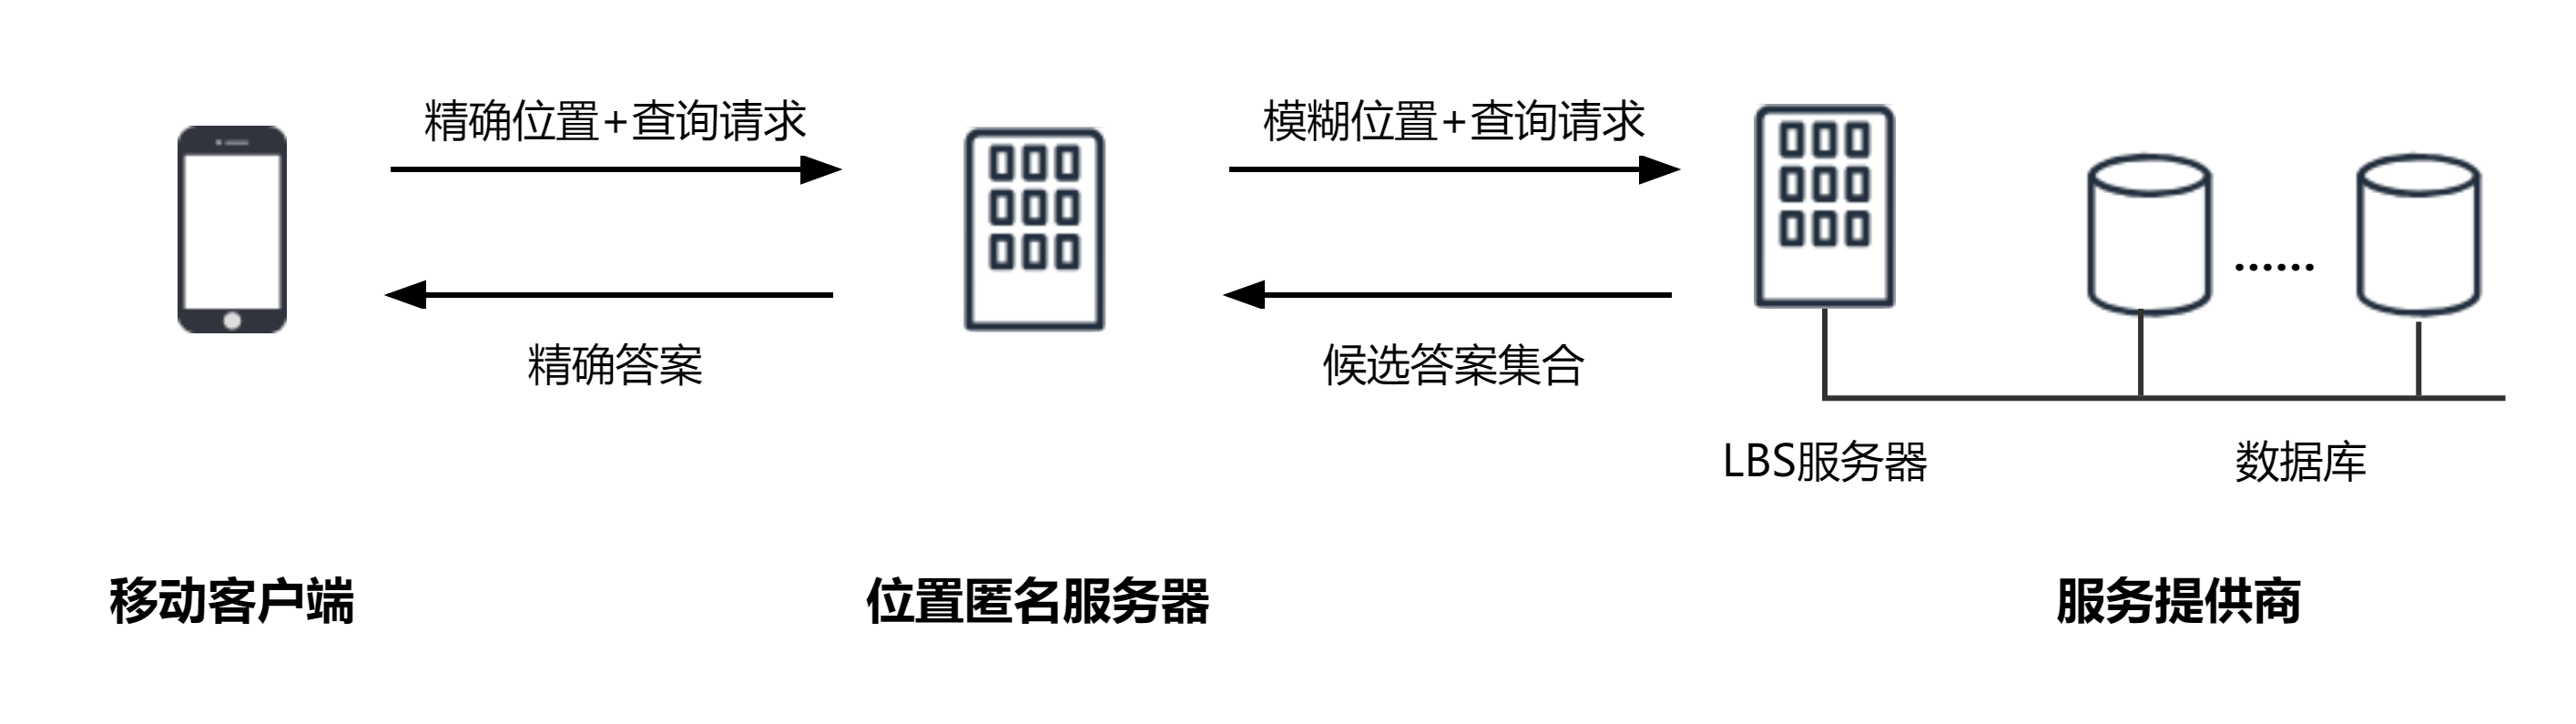
\includegraphics[width=0.8\textwidth]{./include_picture/集中式结构(绪论-研究现状)} %插入图片,[]中设置图片大小,{}中是图片文件名
	\caption{集中式结构系统示意图} %最终文档中希望显示的图片标题
	\label{集中式结构} %用于文内引用的标签
\end{figure}

在集中式结构的位置隐私保护系统中,用户发起查询请求后,由位置匿名服务器对用户的精确位置进行匿名处理。服务提供商受到位置匿名服务器提交的查询请求后,根据接受到的位置返回用户可能需要的答案集合,称为候选答案集合。位置匿名服务器接收到答案集合后,根据用户的精确位置进行筛选求精操作,最终把精确答案返还给用户。$^{[czh\_2.2]}$
\par
引入位置匿名服务器为系统性能带来了显著的提高。一方面,位置匿名服务器承担了位置匿名处理、候选答案求精的任务,从而减轻了用户端的负担,使得用户端的设计可以更为轻量。另一方面,引入位置匿名服务器后,原本一些在移动客户端上难以实现的复杂算法、功能也有了实现的可能,系统功能更加强大。
\par
当然,位置匿名服务器本身也有一些缺点。随着系统的使用,服务器中存储的用户位置数据会逐渐积累。如果没有对服务器存储的数据进行处理,一旦服务器被攻击、或者服务器不再可信,这将会严重损害用户的位置信息隐私安全。此外,当系统用户频繁请求服务时,服务器自身的性能也可能成为限制系统性能的瓶颈。$^{[czh\_2.1]}$


\subsubsection{分布式结构}
鉴于集中结构位置匿名服务器带来的安全问题和性能瓶颈问题,分布式结构去除了位置匿名服务器的存在,而是通过多台移动设备之间的协作来实现位置匿名效果。分布式系统结构示意图见图\ref{分布式结构}。
\begin{figure}[H] %H为当前位置,!htb为忽略美学标准,htbp为浮动图形
	\centering %图片居中
	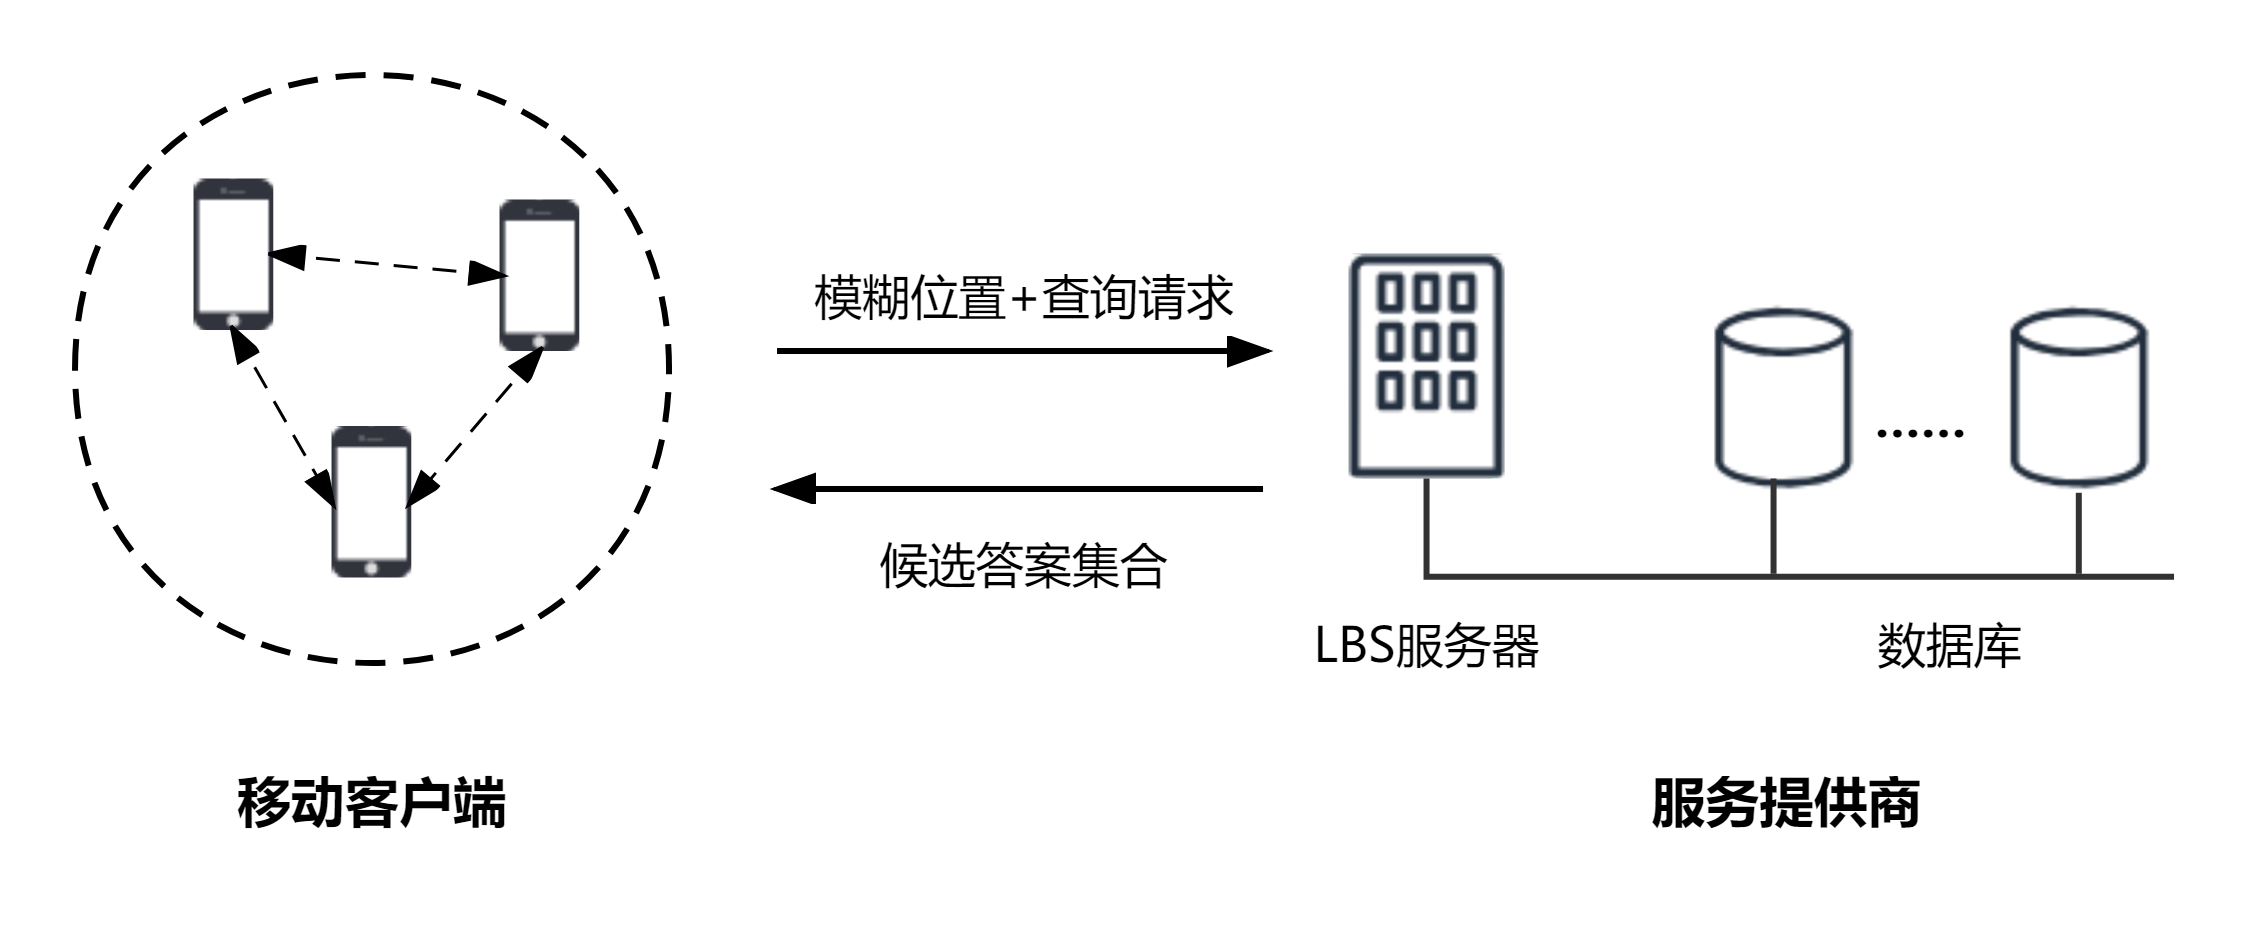
\includegraphics[width=0.8\textwidth]{./include_picture/分布式点对点结构(绪论-研究现状)} %插入图片,[]中设置图片大小,{}中是图片文件名
	\caption{分布式结构系统示意图} %最终文档中希望显示的图片标题
	\label{分布式结构} %用于文内引用的标签
\end{figure}

在分布式结构系统中,用户发起查询请求后,一定区域内的多台移动设备相互协作并进行一定的通信,形成一个匿名区域。服务提供商根据接收到的区域返回相应的候选答案集合,用户接受到答案集合后进行筛选和求取精确答案的操作。
\par
和集中式结构相比,分布式结构的系统进一步降低了用户位置信息泄露的隐患。但分布式结构也对用户移动设备的计算能力提出了一定的要求,以便进行协作匿名。这也限制了分布式结构系统的发展。$^{[czh\_2.1]}$

\subsubsection{混合结构}
考虑到集中式结构系统的计算能力以及分布式结构系统的信息保密性,部分系统融合了上述两种结构,形成了兼具上述优点的新的系统结构——混合结构。混合结构的系统示意图见图\ref{混合结构}。
\begin{figure}[H] %H为当前位置,!htb为忽略美学标准,htbp为浮动图形
	\centering %图片居中
	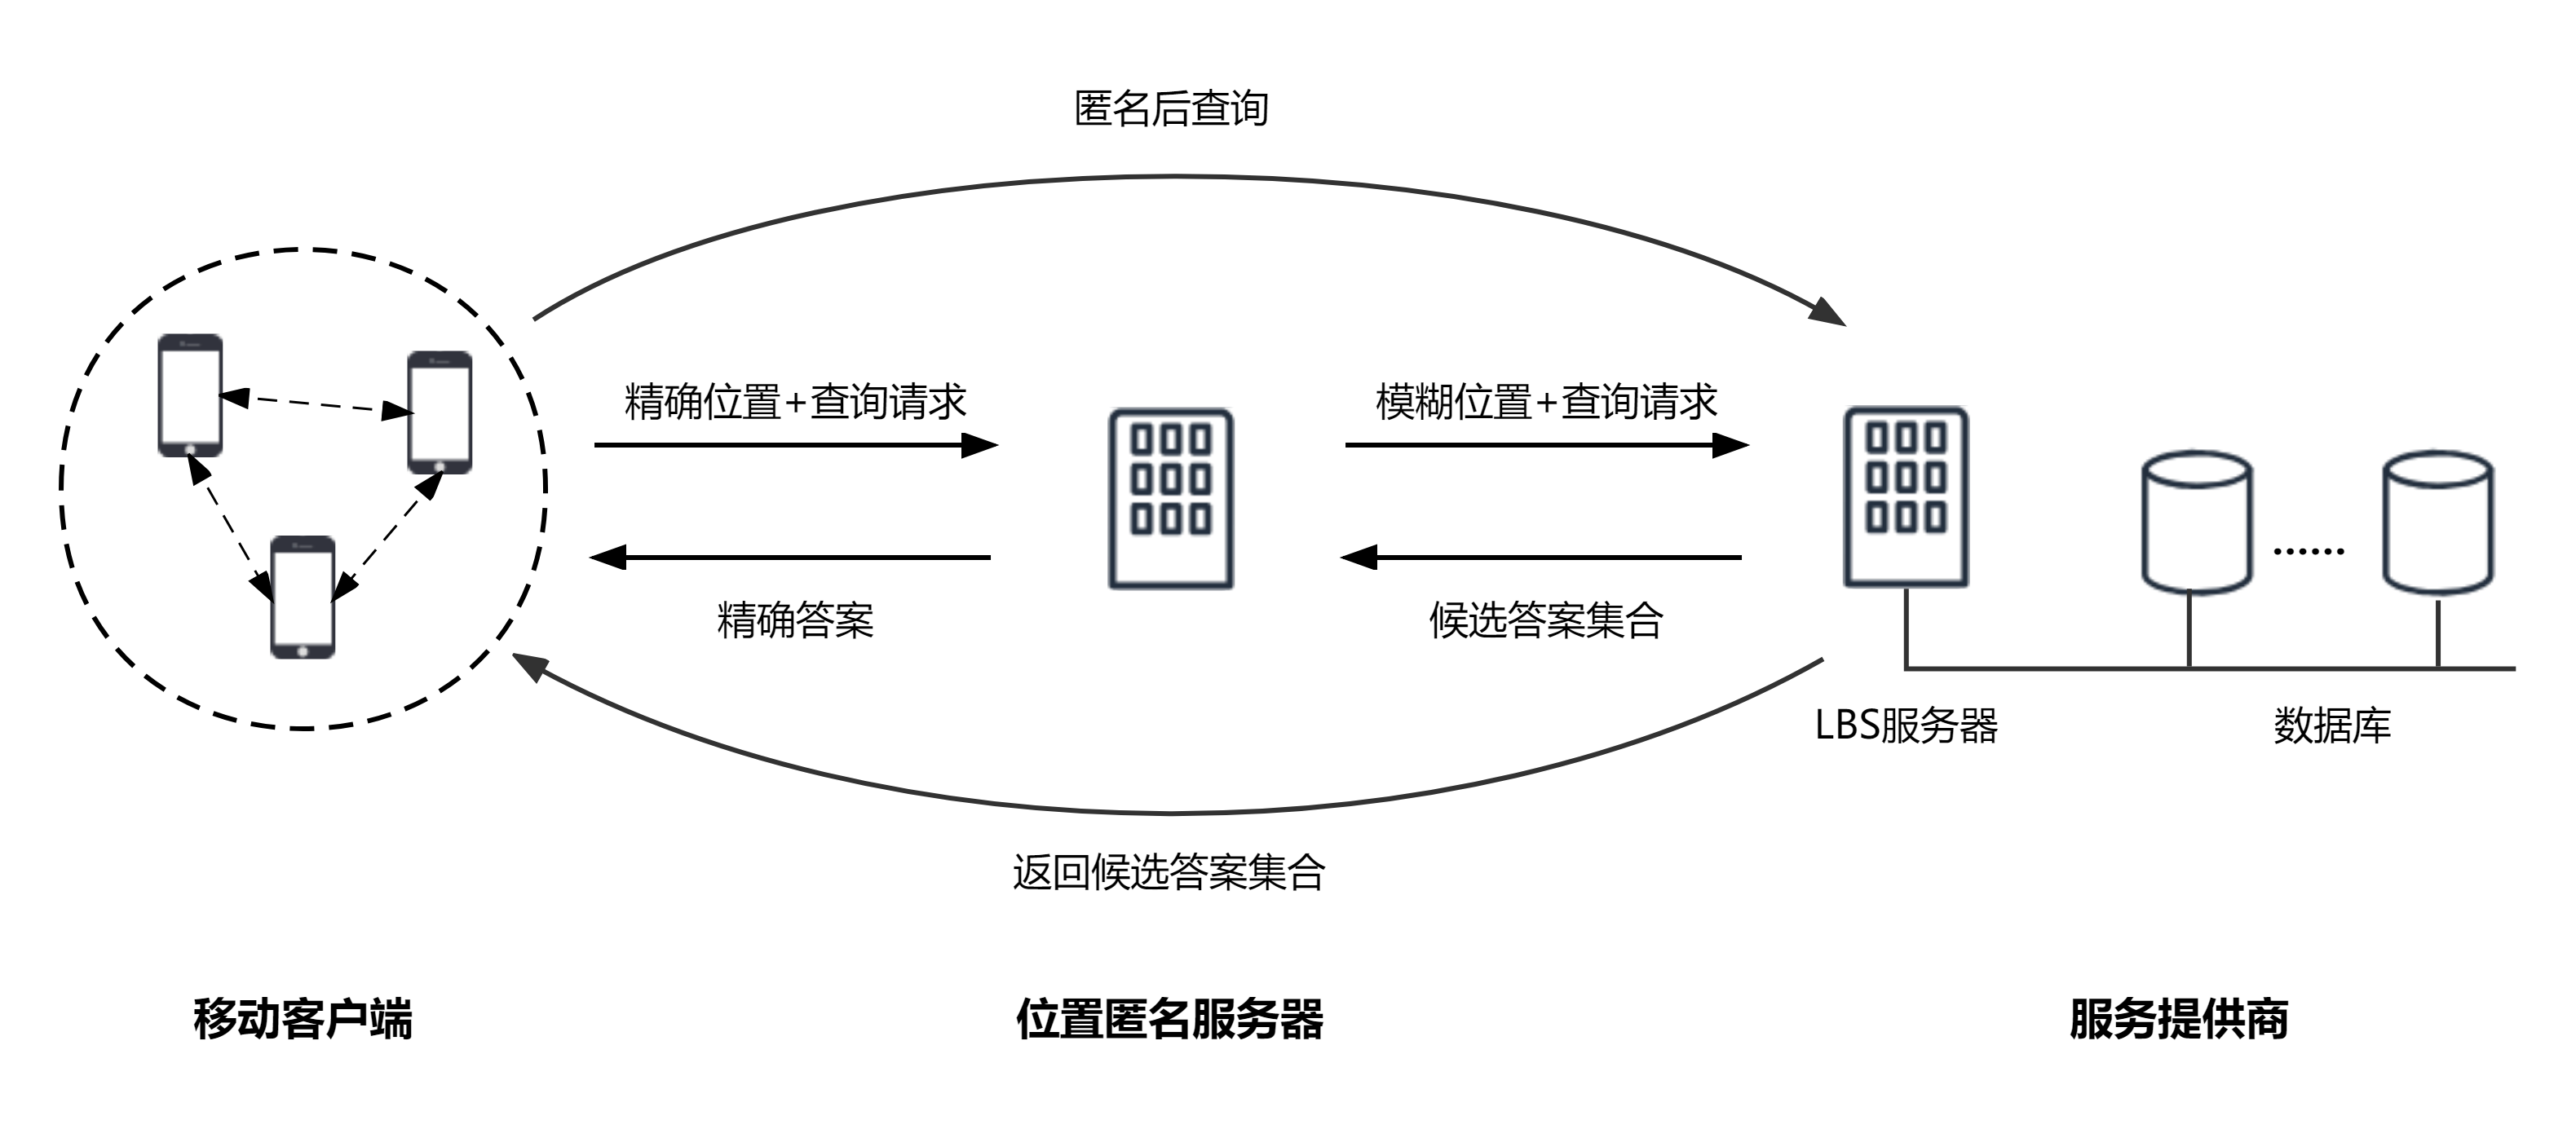
\includegraphics[width=0.8\textwidth]{./include_picture/混合结构(绪论-研究现状)} %插入图片,[]中设置图片大小,{}中是图片文件名
	\caption{混合结构系统示意图} %最终文档中希望显示的图片标题
	\label{混合结构} %用于文内引用的标签
\end{figure}

在混合结构系统中,用户发起查询请求后,系统可以选择让用户通过位置匿名服务器进行匿名查询,也可以联合多台移动设备,通过分布式的方式直接和LBS服务器取得联系,这将取决与系统中发起查询请求的用户数量。
\par
值得一提的是,虽然混合结构吸收了先前两种结构的优点,使它看上去更为灵活。但实际上,在构建和维持混合结构时需要不断设置、调整系统参数,以决定系统什么时候通过哪种方式和LBS服务器建立联系。这也束缚了混合结构的进一步发展$^{[czh\_2.3]}$。
\par \par 
在上面的3个小节中,我们介绍了现行基于位置隐私保护系统的3种主要结构,它们各自的优缺点可以概括为表\ref{3种结构对比}。


\begin{table}[H]
	\caption{位置隐私保护系统3种结构对比}
	\centering
	\label{3种结构对比}
	\begin{tabular}{ccc}
		\hline  
		\makebox[0.1\textwidth][c]{结构名称} & \makebox[0.4\textwidth][c]{优点} & \makebox[0.4\textwidth][c]{缺点}  \\ 
		\hline  
		集中式结构	&	计算、存储性能提高	&	有泄露隐私的风险\\
		分布式结构	&	提高安全性		   &	对移动设备性能要求较高\\
		混合结构	 &	兼具安全性和性能	 & 		系统参数限制了应用\\
		\hline
	\end{tabular} 
\end{table} 


在以上3中位置隐私保护结构的基础上,国内外学者研发出了多种位置隐私保护技术。其中比较著名的有将用户位置信息隐藏在虚拟位置中的\textbf{K-匿名技术}$^{[czh\_2.4]}$,在真实位置信息中添加虚假信息的\textbf{虚假位置技术}$^{[czh\_2.5]}$等等。由于本文主要在系统结构进行创新,这些技术不再一一说明。

\iffalse
\subsubsection{位置隐私保护常用策略(to be merged)}
2.1 虚拟位置策略: \par

\subsubsection{位置隐私保护常用策略}
4.1 虚拟位置策略: \par

通过对用户的精确位置进行泛化处理,向服务提供商提供一个不精确的位置范围,从而保护用户的位置隐私。
对位置进行模糊化有如下集中常用方法:
\begin{itemize}
  \item \textbf{通过分布式架构模糊位置}: 通过与周围移动设备协同工作,共同生成一个模糊的位置范围。
  此方法分散了单个设备的计算负担,但依赖周围设备的参与,可能受到恶意参与用户的影响。
  \item \textbf{通过差分隐私模糊位置}: 向用户精确位置添加随机噪声,制定一个模糊范围。此方法适用于防范数据挖掘等场景,但会对用户设备造成较大计算负担,并降低服务准确性。
  \item \textbf{K-匿名模型}:该方法将用户的位置数据与K-1个其他用户的位置数据合并,从而在一个范围内形成K个位置点。
  这些位置点的特征相似,使得服务提供商无法区分哪个位置点是当前用户的真实位置。K-匿名模型与分布式架构相容性好,灵活度也更高,但效果依赖于对K值的合理选择。
\end{itemize}
\par
4.2 匿名通讯策略: \par
用户使用假ID与服务提供商通信,以实现位置信息匿名化。该方法优点是简单易行。
然而,服务提供商仍可以通过分析用户行为模式来识别用户具体身份,达到“去匿名化”的效果。
为确保隐私效果,用户须定期更换ID。
\par
4.3 密码学策略: \par
采用同态加密等密码学技术,使服务提供商在无需解密数据的情况下提供服务。
尽管这种方法可以提供较高程度的隐私保护,但同态加密等密码算法的计算开销较大,会对用户体验造成负面影响。

\subsubsection{我们的技术}
在实际使用场景中,常常是上述几种位置隐私保护策略的综合,是服务准确性与位置隐私性间的平衡。
我们意识到位置隐私不是用户单方面的权益,在较多情景下,用户不能随机修改其提供的地理位置,
在保护准确位置隐私的同时,也要保证提供的位置是真实的,即位置模糊的同时需要真实。
\par
比如,交友软件中服务提供商需要用户提供相对准确位置以提供服务,而用户则有保护精确位置隐私的需求。
再如,部分互联网服务需要特定地域访问,服务提供商需要确定用户没有造假。
在这些情境下,服务提供商不信任用户自身对精确位置的模糊化处理,不排除用户造假可能。
随着移动设备算力提高,现行技术基本不再使用可信第三方计算中心对位置数据进行匿名模糊化,
转而在本地或直接处理或通过P2P式网络分布式处理,这些隐私保护方法高效可行,但缺乏对用户本身的约束,无法建立起用户和服务提供商间相互信任。
\par
所以我们引入“零知识证明”
具体流程如下:
\begin{itemize}
  \item 
\end{itemize}
\fi 


\subsection{研究内容与贡献(to be continued)}

\subsection{章节安排(to be continued)}

\subsection{前景扩展(to be merged)}
兴趣点(Point of Interest)分析:【引用】
兴趣点指的是用户周边地理实体,包括餐馆酒店、娱乐场所、商超银行、地铁公交等,可能是用户潜在感兴趣的消费地点。
服务提供商通过分析用户位置的周边信息,满足用户查询需求。

社交娱乐:交友软件,同城社交分享:
同城摇一摇,同城交友

精确广告服务:
广告商通过对用户精确位置和活动轨迹的分析,向用户投放精准定制化的广告,尤其是向用户推荐周边商户和服务。
周边位置的购物折扣、餐饮娱乐和房屋租赁等广告可以很好切中用户需求,拉近周边商户与用户举例。


\section{基础概念与预备知识}\label{基础概念与预备知识}
\subsection{非负矩阵分解}
\subsubsection{概念}
非负矩阵是指每一个元素都是非负实数的矩阵。1999年Lee等人$^{[czh\_3.1]}$提出非负矩阵分解(Non-negative Matrix Factorization,NMF)算法,可以在丢失信息较少的条件下,对高维矩阵数据进行压缩,从而获得稠密的向量或数据。
\par 
给定$n \times m$维的数据矩阵$X \in \mathbb{R}^{n \times m}_+$,m代表数据样本数量,X中每一个列向量代表一个样本数据。$^{[czh\_3.2]}$NMF算法可以将高维矩阵X分解为两个低维非负矩阵,即

\begin{equation}\label{非负矩阵分解1}
	X \approx W H
\end{equation}

其中$W \in \mathbb{R}^{n \times r}_+, H \in \mathbb{R}^{r \times m}_+$分别代表系数矩阵、基矩阵。
一般情况下r远小于n,即$r \times (m+n) < n \times m$。所以可以在基本保存原有数据特性的基础上,把原始矩阵压缩为系数矩阵,从而降低矩阵维数。

\subsubsection{算法简介}
NMF算法有两种常用的求解方式,分别是基于欧氏距离(Euclidian Distance, ED)的\textbf{Frobenius范数}和\textbf{广义KL散度}(Generalized Kullback-Leibler Divergrnce, GKLD)。以Frobenius范数的求解形式为例。
\par 
该算法需要最小化等式\ref{非负矩阵分解2}中目标函数。

\begin{equation}\label{非负矩阵分解2}
	F_{NMF} = \frac{1}{2} \| X - WH \|^2 _F = \frac{1}{2} \sum_{ij}(X_{ij} - WH_{ij})^2
\end{equation}

其中$X_{ij}$表示矩阵X中第i行第j列的元素,$\| \cdot \|^2_F$表示矩阵的Frobenius范数。
\par 
目标函数的迭代规则为:

\begin{equation}\label{非负矩阵分解3}
	W_{ik} \leftarrow W_{ik} \frac{XH^T_{ik}}{WHH^T_{ik}}
\end{equation}

\begin{equation}\label{非负矩阵分解4}
	H_{kj} \leftarrow H_{kj} \frac{W^TX_{kj}}{W^THH_{kj}}
\end{equation}	

其中$i = 1,2\cdot \cdot \cdot n; j = 1,2\cdot \cdot \cdot m$。给定迭代终止条件后,对随机生成的初始非负矩阵$W_0,H_0$按式子\ref{非负矩阵分解3}和式子\ref{非负矩阵分解4}中的迭代规则交替迭代,直到满足终止条件,即可得到需要的W和H。$^{[czh\_3.3]}$

\subsection{地理近邻矩阵}\label{地理近邻矩阵}
在基于位置的社交网络(Location Based Social Network, LBSN)中,用户签到的地点被称为兴趣点(Point-of-Interest, POI)。通常位置临近的兴趣点被共同访问的可能性比较高,因此不同兴趣点在地理位置上的临近性成为了当前基于位置信息进行个性化推荐的一个重要指标。
\par 
为了描述不同兴趣点之间的地理临近性,本文引入一个地理近邻矩阵$^{[czh\_4.1]}$,并设置一个距离阈值s来刻画不同兴趣点之间的地理近邻性。矩阵中第i行第j列的元素$g_{ij}$表示第i个兴趣点和第j个兴趣点之间的近邻性。若i和j两个兴趣点之间的距离在区间[0, s]之间,则$g_{ij}=1$;否则$g_{ij}=0$。规定$g_{ii}=1$,即矩阵对角线上的元素为1。
\par 
地理近邻矩阵将在本文第\ref{作品设计与实现}章第\ref{关键技术}节中的地理信息模型中进行应用。

\section{作品设计与实现}\label{作品设计与实现}
\subsection{系统概述}
\subsection{关键技术}\label{关键技术}
\subsubsection{基于非负矩阵分解的兴趣点推荐模型}
在本文的位置隐私保护系统中,服务提供商初次返回分布在随机位置的若干服务,接着移动用户端对这些服务所代表的位置进行零知识范围证明,判断哪些服务的位置在用户所能接受的地理范围内,并将可以接受的位置返还给服务提供商。接下来,服务提供商就需要根据这些返回的位置,决定自己接下来要向用户提供哪些服务。
\par 
所以这一阶段服务提供商需要解决的问题可以转化为:已知若干个兴趣点(POI)的位置,如何根据已有兴趣点的位置,判断出用户可能想要前往的兴趣点?
\par 
考虑到大多数人的移动能力和行进心理,用户通常喜欢访问距离当前位置较近的兴趣点。为此,我们引入在本文第\ref{基础概念与预备知识}章第\ref{地理近邻矩阵}节所提到的\textbf{地理近邻矩阵},在此基础上构建兴趣点推荐模型,来刻画不同兴趣点之间在地理上的近邻性,进而反映用户访问的不同兴趣点可能性的不同,达到为进行用户个性化推荐的效果。
\par 
下面将用一组简单数据来演示基于非负矩阵分解的地理信息模型。表\ref{经纬度}是各POI的经纬度,由此求出的各POI的地理距离如表\ref{距离}所示。假如我们设置距离阈值 s=80 km,则可以进一步求出表\ref{矩阵表}的地理近邻矩阵。


\begin{table}[H]
	\centering
	\begin{minipage}{0.3\textwidth}
		\centering
		\small
		\makeatletter\def\@captype{table}\makeatother
		\caption{各POI经纬度} 
		\label{经纬度}
		\begin{tabular}{ccc}
			\hline
			POI & Latitude & Longitude \\
			\hline
			a & 39.5856 & 116.2041  \\
			b & 40.0000 & 116.1221 \\
			c & 39.5567 & 116.8354  \\
			d & 39.0100 & 115.8324 \\
			\hline
		\end{tabular}
	\end{minipage}\quad
	\begin{minipage}{0.3\textwidth}
		\centering
		\small
		\makeatletter\def\@captype{table}\makeatother
		\caption{各POI距离(km)} 
		\label{距离}
		\begin{tabular}{|c|c|c|c|c|}
			\hline
			& a & b & c & d \\
			\hline
			a & 0 	& 46.6 & 54.2 & 71.6  \\
			\hline 
			b & 46.6 & 0	& 78.4 & 112.9  \\
			\hline 
			c & 54.2 & 78.4 & 0 	& 105.6  \\
			\hline 
			d & 71.6 & 112.9 & 105.6 	& 0  \\
			\hline 
		\end{tabular} 
	\end{minipage}\quad
	\begin{minipage}{0.3\textwidth}
		\centering
		\small
		\makeatletter\def\@captype{table}\makeatother
		\caption{地理近邻矩阵}
		\label{矩阵表}
		\begin{tabular}{|c|c|c|c|c|}
			\hline
			& a & b & c & d \\
			\hline
			a & 1 & 1 & 1 & 1  \\
			\hline 
			b & 1 & 1 & 0 & 0  \\
			\hline 
			c & 1 & 0 & 1 & 0  \\
			\hline 
			d & 1 & 0 & 0 & 1  \\
			\hline 
		\end{tabular} 
	\end{minipage}
	\vspace{-5pt}
\end{table}

经过上述步骤,我们已经构造出了地理近邻矩阵。但是还需要注意到,现实生活中各种服务在地理位置上并不是均匀分布,所以经过以上步骤得到的地理近邻矩阵实际上是一个相当稀疏的矩阵。如果直接将这个矩阵融入我们的兴趣点推荐模型,得到的推荐结果效果会有巨大的提升空间。
\par 
为了充分利用兴趣点在地理上的近邻特征,本文采用非负矩阵分解的方法,对得到的地理近邻矩阵进行降维处理,使兴趣点的位置信息从稀疏的高维向量转化为稠密的低维向量,方便后续操作。具体的,可以把上述得到的地理近邻矩阵$G \in \mathbb{N}^{N \times N}$
分解成基矩阵$E_g \in \mathbb{R}^{N \times d_g}$
和系数矩阵$H_g \in \mathbb{R}^{d_g \times N}$,实现降维处理,即

\begin{equation}
	G \approx E_g H_g
\end{equation}

本文使用基于Frobenius范数的损失函数,函数计算公式如下式\ref{损失函数}所示$^{[czh\_4.1]}$。其中$d_g\text{是}E_g$中隐向量的维度,$\| \cdot\|_F$是矩阵Frobenius范数,$\| \cdot\|_1$是$L_1$范数,
$\partial _g$是$L_1$和$L_2$正则化参数,$\rho _g$是$L_1$正则化占总正则化的比例。公式中的误差优化通过随机梯度下降实现。

\begin{equation}
	\label{损失函数}
	\begin{aligned}
		\underbrace{arg\, min}_{W_g, H_g} \frac{1}{2} \bigg[ \|G-E_gH_g\|^2_F + 
		\partial _g \rho _g \|E_g\|_1 + \partial _g \rho _g \|H_g\|_1 \\
		+ \frac{\partial _g(1-\rho _g)}{2}\|E_g\|^2_F 
		+ \frac{\partial _g(1-\rho _g)}{2}\|H_g\|^2_F  \bigg]
	\end{aligned}
\end{equation}

完成分解后,$E_g$的行向量即为兴趣点的地理近邻特征向量。对于多个兴趣点,即便它们之间不存在直接意义上的地理近邻性,非负矩阵分解也可以得出它们之间间接的近邻性,从而为兴趣点推荐提供判断依据。


%********************格式要求********************
\section{简介}
\setParDis %设置段间距为 0
\begin{spacing}{1.5}
  第三十三届“冯如杯”主赛道论文一律由在计算机上输入、排版、定稿后转成PDF格式,
在集中申报时通过网络上传。\textbf{论文封面及全文中不能出现作者姓名、学院、专业、指导老
师的相关信息}。包括5个部分, 顺序依次为: \par 
  % 段落间可加入\par进行换行,代替两行回车的写法
  \begin{itemize}
    \item 封面(中文)
    \item 中文摘要、关键词(中文、英文)
    \item 主体部分
    \item 结论
    \item 参考文献
  \end{itemize}

\section{论文的书写规范}

论文正文部分需分章节撰写,每章应另起一行。
章节标题要突出重点,简明扼要、层次清晰。字数一般在15字以内,不得使用标点符号。标题中尽量不采用英文缩写词,对必须采用者,应使用本行业的通用缩写词。  层次以少为宜,根据实际需要选择。三级标题的层次按章(如“一、”)、节(如 “(一)”)、条(如“1.”)的格式编写,各章题序的阿拉伯数字用 Times New Roman 体。  

\subsection{字体和字号}
论文题目:二号,华文中宋体加粗,居中。

副标题:三号,华文新魏,居右(可省略)。

章标题:三号,黑体,居中。

节标题:四号,黑体,居左。

条标题:小四号,黑体,居左。

正文:小四号,中文字体为宋体,西文字体为Times New Roman体,首行缩进,两端对齐。

页码:五号Times New Roman 体,数字和字母\par

\subsection{页边距及行距}
学术论文的上边距:25mm;下边距:25mm;左边距:30mm;右边距 20mm。
章、节、条三级标题为单倍行距,段前、段后各设为0.5行(即前后各空0.5行)。
正文为 1.5 倍行距,段前、段后无空行(即空0行)。

\subsection{页眉}
页眉内容为北京航空航天大学第三十三届“冯如杯”竞赛主赛道参赛作品,内容居中。
页眉用小五号宋体字,页眉标注从论文主体部分开始(引言或第一章)。
请注意论文封面无页眉。

\subsection{页码}
论文页码从“主体部分(引言、正文、结论)”开始,直至“参考文献”结束,用五号阿
拉伯数字连续编码,页码位于页脚居中。\textbf{封面、题名页不编页码。}

摘要、目录、图标清单、主要符号表用五号小罗马数字连续编码,页码位于页脚居中。

\subsection{图、表及其附注}
图和表应安排在正文中第1次提及该图、表的文字的下方,当图或表不能安排在该页时,
应安排在该页的下一页。

\subsubsection{图}
图题应明确简短,\textbf{用五号宋体加粗},数字和字母为\textbf{五号Times New Roman体
加粗},图的编号与图题之间应空半角2格。图的编号与图题应置于图下方的居中位置。图内文字
为\textbf{5号宋体},数字和字母为\textbf{5号Times New Roman体}。曲线图的纵横坐标必
须标注“量、标准规定符号、单位”,此三者只有在不必要注明(如无量刚等)的情况下方可省略。
坐标上标注的量的符号和缩略词必须与正文中一致。

\subsubsection{表}
表的标号应采用从1开始的阿拉伯数字编号,如:“表 1”、“表 2”、……。表编号应一直连续到附录
之前,并与章、节和图的编号无关。只有一幅表,仍应标为“表 1”。表题应明确简短,用\textbf{五号宋体
加粗},数字和字母为\textbf{五号Times New Roman体加粗},表的编号与表题之间应空半角2格。表的编号与
表头应置于表上方的居中位置。表内文字为\textbf{5号宋体},数字和字母为\textbf{5号Times New Roman体}。  

\subsubsection{附注}
图、表中若有附注时,附注各项的序号一律用“附注+阿拉伯数字+冒号”,如:“附注1:”。

附注写在图、表的下方,一般采用5号宋体。

\subsubsection{参考文献}
凡有直接引用他人成果(文字、数字、事实以及转述他人的观点)之处,均应加标注说明列于参考文献中,
以避免论文抄袭现象的发生。

标注格式:引用参考文献标注方式应全文统一,标注的格式为[序号],放在引文或转述观点的最后
一个句号之前,所引文献序号用小4号Times New Roman体、以上角标形式置于方括号中,如“……成果”$^{[1]}$。
\section{公式模板}

公式示例展示如下:
\begin{align}
\underset{{\bf I}_c \sim \boldsymbol\Im_c}{\mathrm{\text P}} \Big( \mathcal C({\bf I}_c) \neq \mathcal C({\bf I}_c + \boldsymbol \rho) \Big) \geq \delta ~~~\text{s.t.}~~||\boldsymbol\rho||_p \leq \xi,
\label{eq:def1}
\end{align}

\section{图表模板}
图表示例展示如下:

%插入一张图片
\begin{figure}[H] %H为当前位置,!htb为忽略美学标准,htbp为浮动图形
    \centering %图片居中
    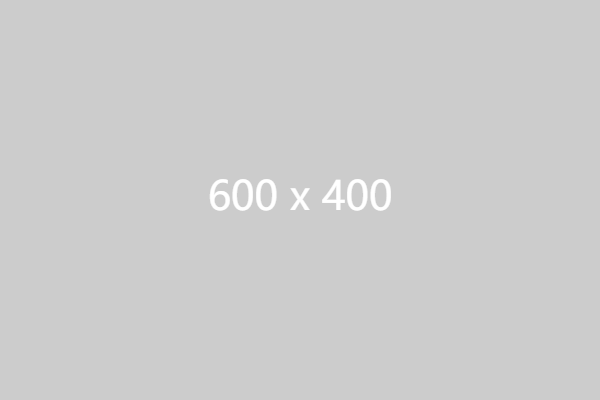
\includegraphics[width=0.8\textwidth]{example-image-2.png} %插入图片,[]中设置图片大小,{}中是图片文件名
    \caption{example\_caption} %最终文档中希望显示的图片标题
    \label{example_label} %用于文内引用的标签
\end{figure}

% 一行三张子图并排示意
\begin{figure}[htbp]
  \begin{subfigure}{0.31\textwidth}
    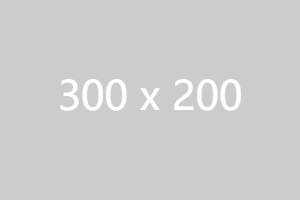
\includegraphics[width=\linewidth]{example-image-1.png}
    \caption{示意图1} \label{fig:9aaa}
  \end{subfigure}%
  \hspace*{\fill}   % maximize separation between subfigures
  \begin{subfigure}{0.31\textwidth}
    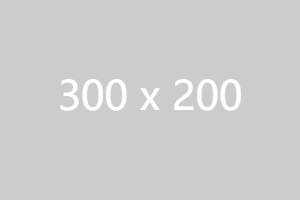
\includegraphics[width=\linewidth]{example-image-1.png}
    \caption{示意图2} \label{fig:9bbb}
  \end{subfigure}
  \hspace*{\fill}   % maximizeseparation between subfigures
  \begin{subfigure}{0.31\textwidth}
    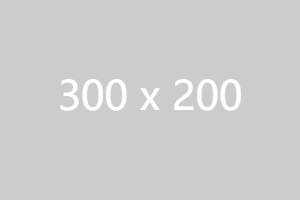
\includegraphics[width=\linewidth]{example-image-1.png}
    \caption{示意图3} \label{fig:9ccc}
    \end{subfigure}
\caption{一行三张子图并排示意}
\label{qmix-train}
\end{figure}


% 2*2四张子图示意
\begin{figure}[htbp]
  \begin{subfigure}{0.48\textwidth}
    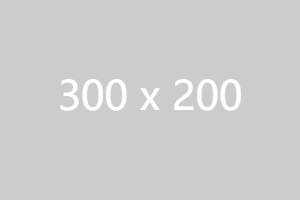
\includegraphics[width=\linewidth]{example-image-1.png}
    \caption{示意图1} \label{fig:8a}
  \end{subfigure}%
  \hspace*{\fill}   % maximize separation between subfigures
  \begin{subfigure}{0.48\textwidth}
    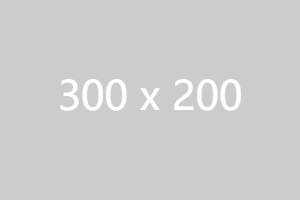
\includegraphics[width=\linewidth]{example-image-1.png}
    \caption{示意图2} \label{fig:8b}
  \end{subfigure}\\
  %\hspace*{\fill}   % maximizeseparation between subfigures
  \begin{subfigure}{0.48\textwidth}
    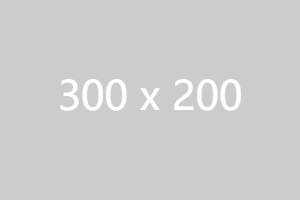
\includegraphics[width=\linewidth]{example-image-1.png}
    \caption{示意图3} \label{fig:8c}
  \end{subfigure}
  \hspace*{\fill}   % maximize separation between subfigures
  \begin{subfigure}{0.48\textwidth}
    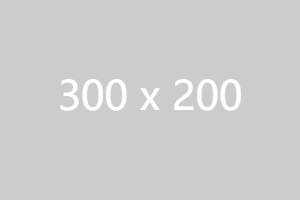
\includegraphics[width=\linewidth]{example-image-1.png}
    \caption{示意图4} \label{fig:8d}
  \end{subfigure}
\caption{2*2四张子图示意} \label{fig:8}
\end{figure}

%插入一个表格

\begin{table*}[t]
\centering
\caption{表格使用示例}
\begin{tabular}{|l||c|c|c|c|c|c|}
\hline
{\textbf{表头 1}}     &  表头 2 	    & 表头 3 	  & 表头 4     & 表头 5 		\\ \hline\hline
内容 11 		          & 内容 12				& 内容 13		& 内容 14 	 & 内容 15		\\ \hline
内容 21	              & 内容 22				& 内容 23		& 内容 24	   & 内容 25		\\ \hline


\end{tabular}
\end{table*}


%再插入另一种表格
\begin{table}[H]
\caption{三线表使用示例}
\centering
\begin{tabular}{ccccc}
\hline  
\textbf{方法} & \textbf{表头 1} & \textbf{表头 2} & \textbf{表头 3} & \textbf{表头 4} \\ 
\hline  
方法1 & 数据  & 数据  & 数据  & 数据\\
方法2 & 数据  & 数据  & 数据  & 数据\\
\hline
\end{tabular} 
\end{table} 

\section*{结论}% section*生成无标号章节
\addcontentsline{toc}{section}{结论} % 将无标号章节添加至目录
论文的结论单独作为一章,但不加章号。

注意: 文件大小不超过5M。

\end{spacing}

\newpage

% XSP 2023/3/16: bib支持不全,暂时改为手动
\section*{参考文献} % section*生成无标号章节题目
\addcontentsline{toc}{section}{参考文献} % 将无标号章节添加至目录
% 著作: [序号]作者.书名[标识码].出版地:出版社,出版年.
[1]张志建.严复思想研究[M].桂林:广西师范大学出版社,1989. 

% 译著: [序号]国名或地区(用圆括号)原作者.书名[标识码].译者.出版地:出版社,出版年.
[2](英)霭理士.性心理学[M].潘光旦译.北京:商务印书馆,1997.

% 古典文献 文史古籍类引文后加序号,再加圆括号,内加注书名、篇名

% 论文集: [序号]编者.书名[标识码].出版地:出版社,出版年.
[3]伍蠡甫.西方论文选(下册)[C].上海:上海译文出版社,1979.

% 期刊文章: [序号]作者.篇名[标识码].刊名,年,(期).
[4]叶朗.《红楼梦》的意蕴[J].北京大学学报(哲学社会科学版),1989,(2)

% 报纸文章: [序号]作者.篇名[标识码].报纸名,出版日期(版次)
[5]谢希德.创造学习的新思路[N].人民日报,1998-12-25(10)

% 外文文献: 要求外文文献所表达的信息和中文文献一样多,但文献类型标识码可以不标出。
[6]Mansfeld, R.S. \& Busse. \textit{T.V. The Psychology of creativity and discovery}, Chinago:
NelsonHall, 1981




% \begingroup
% \setstretch{2.0}    %行距2
% \setlength{\bibsep}{0pt}    %段前段后0
% \begin{adjustwidth}{0.42cm}{0.42cm} %左右缩进0.42cm
% \bibliography{references}
% \end{adjustwidth}
% \endgroup

\end{document}
